\documentclass{article}
\usepackage{polski}
\usepackage[utf8]{inputenc}
\usepackage{mathtools}
\usepackage{graphicx}

\graphicspath{{../img/}}

\begin{document}

\section{Data Generation}

  I decided to implent data generator myself (code can be found in the zip archive attached).
  The basic idea for circular and ring data set was generating random radius (within the range) and
  angle theta (within 2 $\pi$ range).

The sets looked like this:

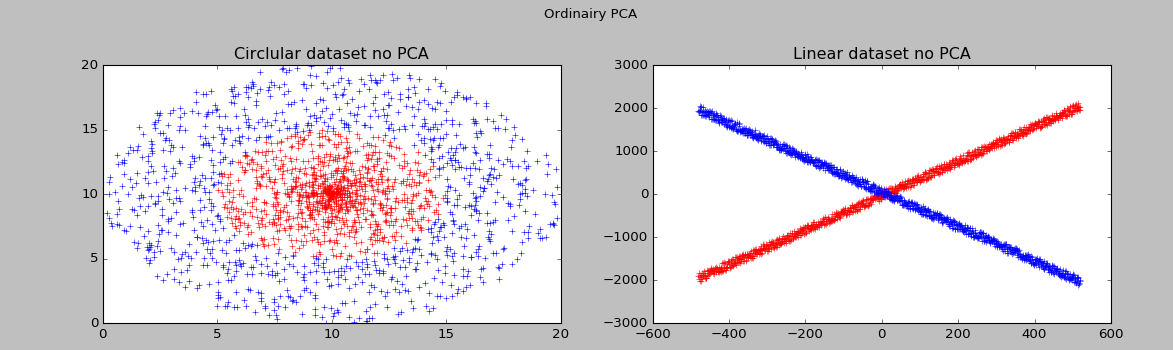
\includegraphics[width=\textwidth]{basic_sets}

\section{Applying basic PCA}

Next basic Principal Components Analysis algorithm was applied. After this transformation, the data sets looked like this:

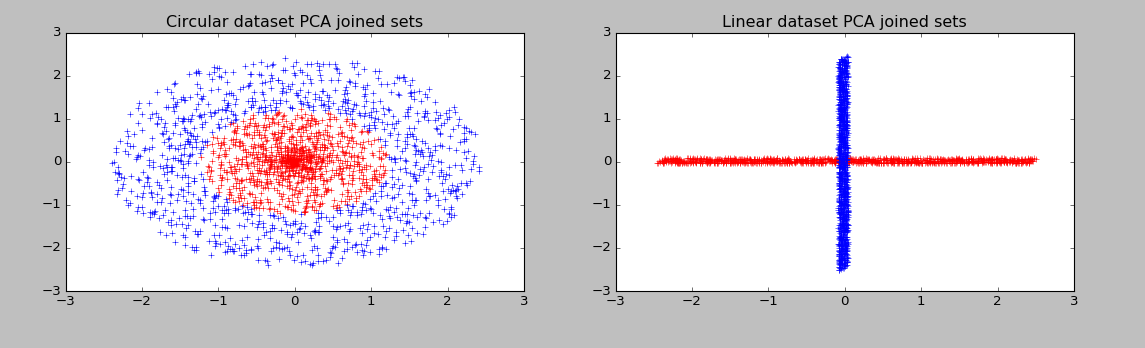
\includegraphics[width=\textwidth]{pca_sets}.

As the plot shows PCA managed to correctly identify most important dimensions in case of linear data,
But failed to make much of a difference with non-linear data.

\section{Applying PCA with kernel trick}

Fortunately there is a way for PCA to perform well on non-linear data: kernel tricks. Kernel tricks is a method of
replacing the basic PCA'a dot product with another function. The problem was the kernel tricks that  I used require
a parameter called gamma. It had to be found by trial and error (otherwise I would need to implement i method like SVM
to evalute how well did PCA with specific value of gamma).

After extensive search for correct gamma parameter I settled down with value 0.1, which gave this results:

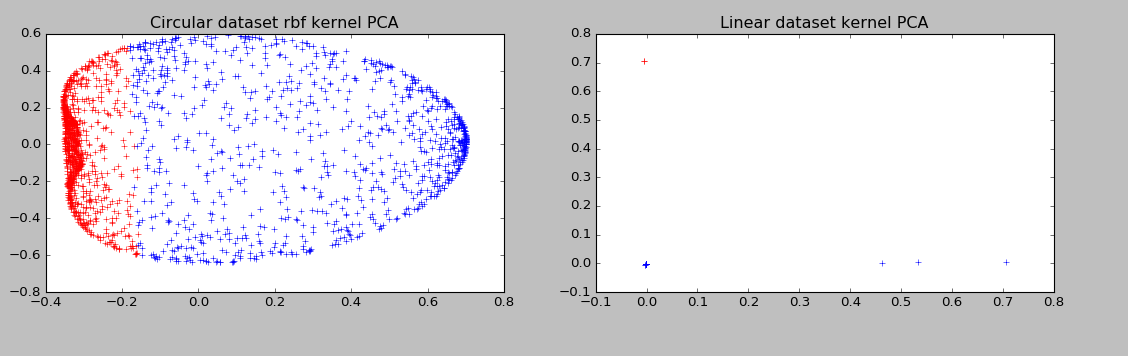
\includegraphics[width=\textwidth]{rbf}

Obviously the set on the left is easily separable by a vertival line ($~x=-0.2$). It also seems that the
linear set was sort of separated, but most probably red crosses are overlapping with blue ones.

Cosine kernel was also pretty successful for the circular data set, but didn't work well for linear dataset:

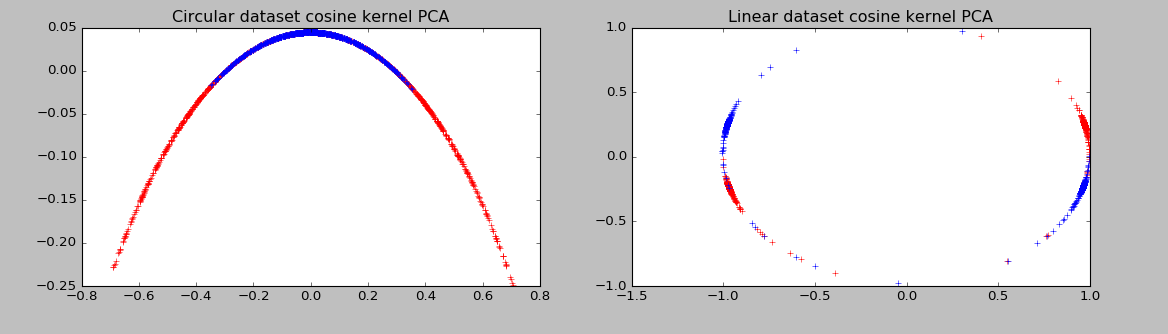
\includegraphics[width=\textwidth]{cosine}

Unfortunately despite testing many values for sigmoid kernel I wasn't able to find any value, with would separate
data sets properly.

These are plots for some of the values I tried:

\subsection{Linear:}

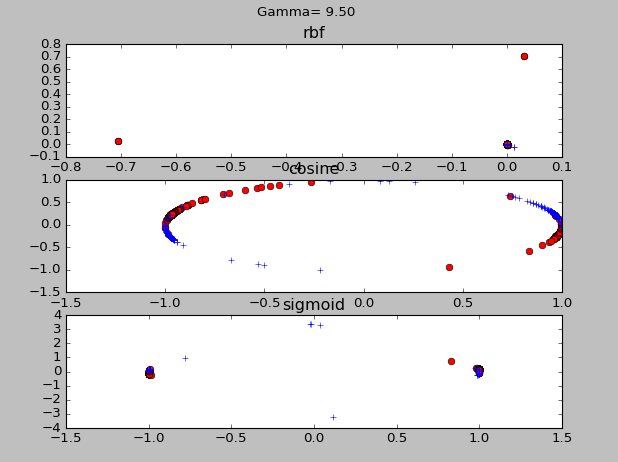
\includegraphics[width=\textwidth]{lin}


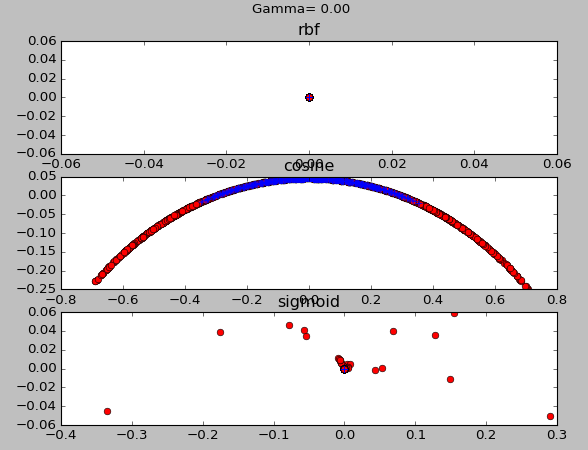
\includegraphics[width=\textwidth]{line}

\subsection{Circular:}

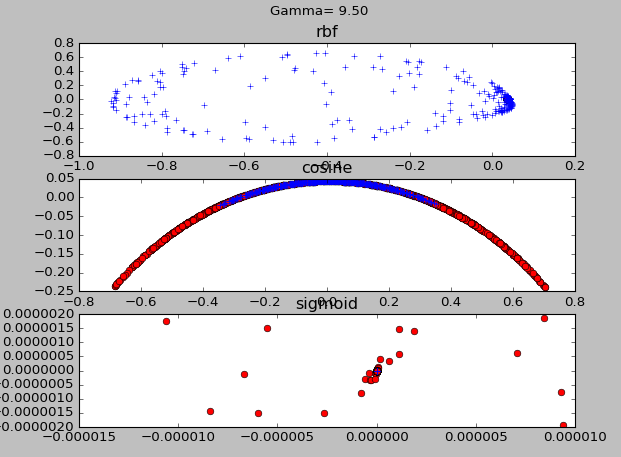
\includegraphics[width=\textwidth]{circ}
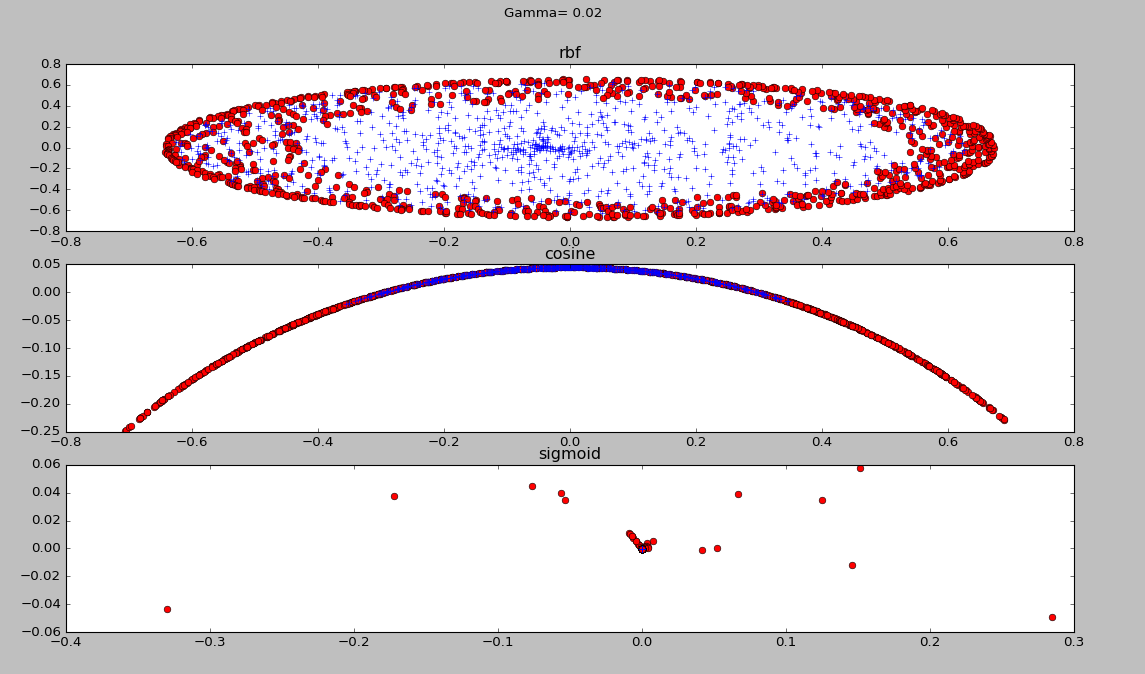
\includegraphics[width=\textwidth]{circu}


\end{document}
